\Huge

\section{The velocity field}

\todo[inline]{Introduce our use of the velocity field to do the reconstruction. Present method of obtaining this in practice and the problems encountered.}

% \begin{figure}
%     \centering
%     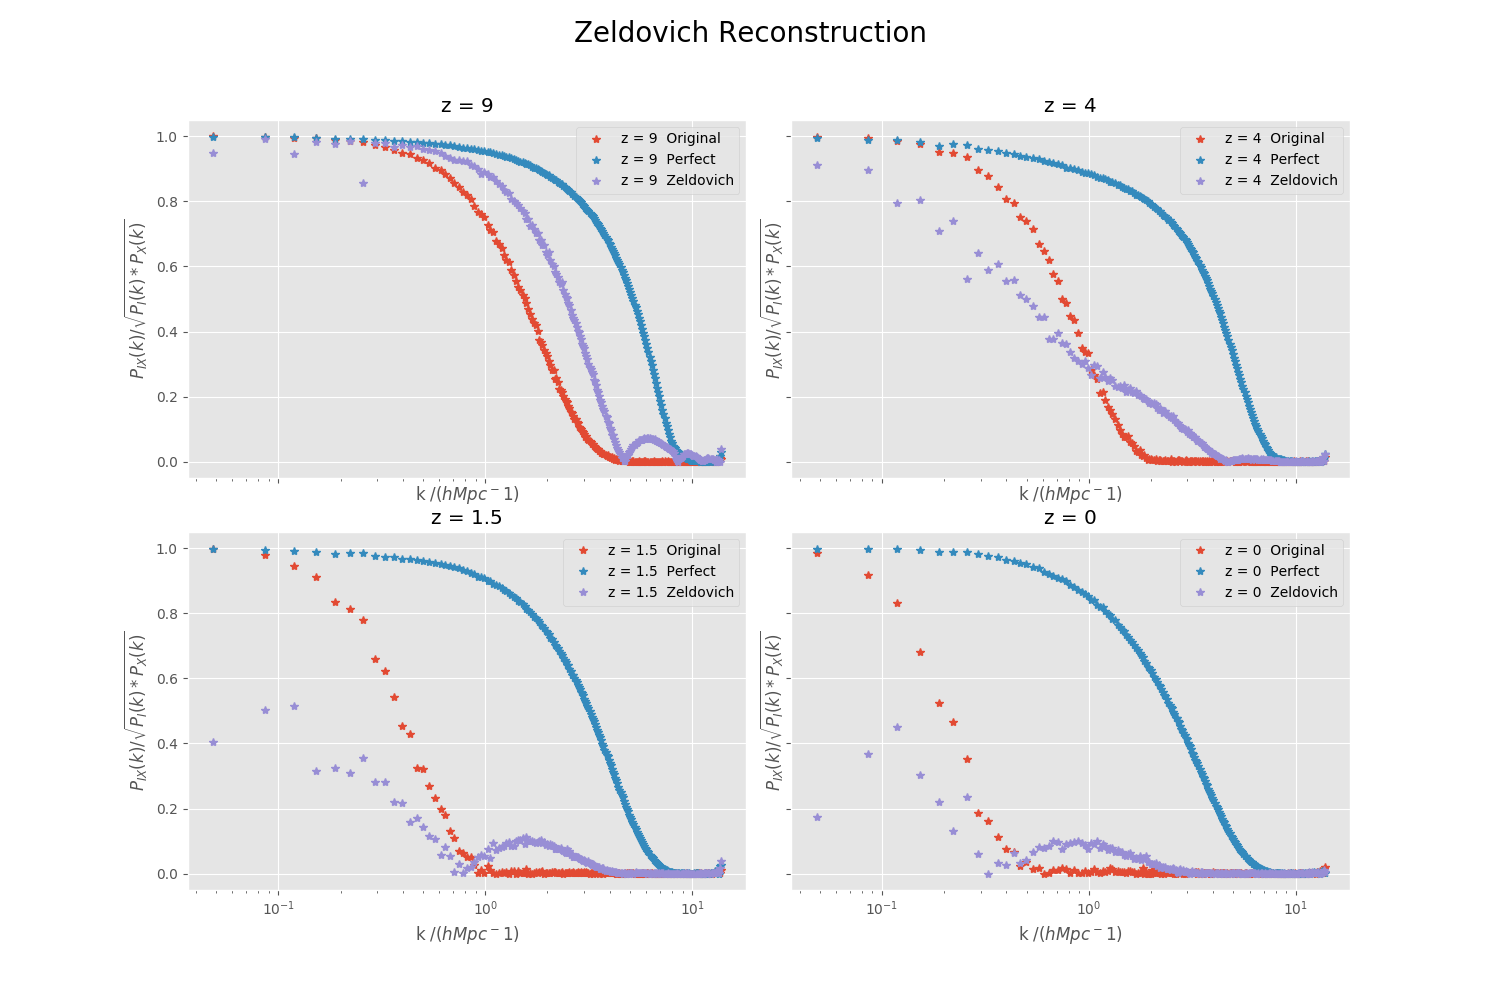
\includegraphics[width=1\columnwidth]{images/crossSpectra/Spec_4_zeld.png}%
    
%     \caption{
%     Reconstructed by applying the Zeldovich Offset directly to the particles for different redshifts.
%     }
    
%     \label{fig:7}
% \end{figure}

\section{Getting back to the linear regime}

\todo[inline]{Talk about how we try to get back to the linear regime. Introduce different ways of avergaing the velocities}

\section{Results}

\todo[inline]{Present our results -> Density Slices and Cross Spectra.}

% \begin{figure}
%     \centering
%     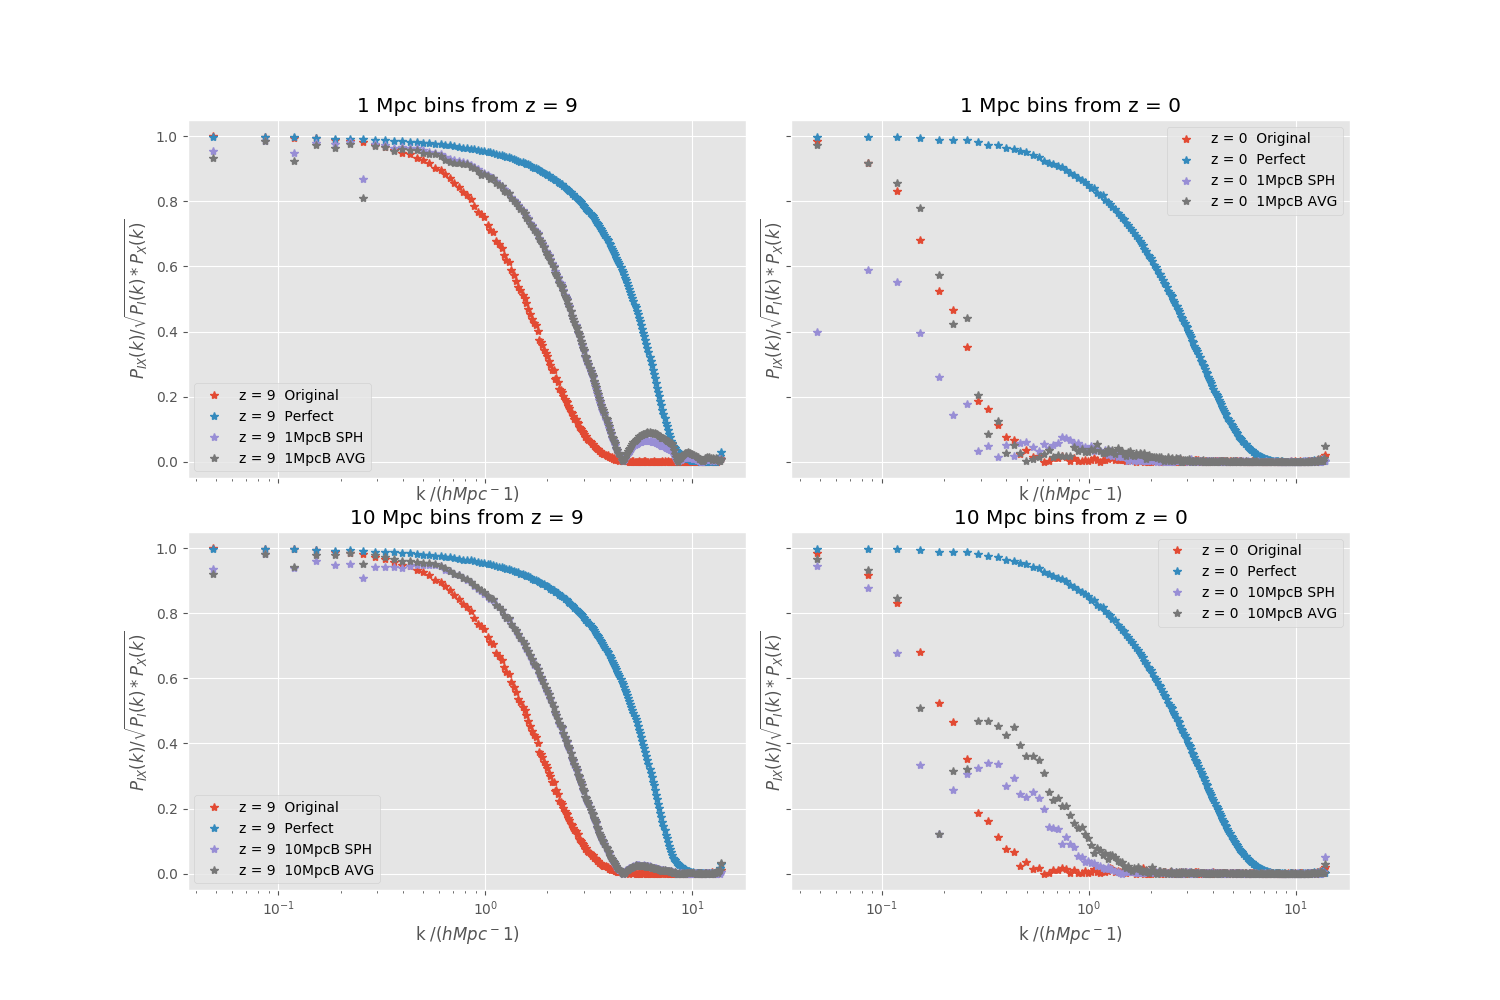
\includegraphics[width=1\columnwidth]{images/crossSpectra/Spec_5_norm.png}%
    
%     \caption{
%     Cross spectra of realistic reconstructions from redshift 9 and 0, using 1 Mpc and 10 Mpc bins to average velocities. There are two averaging methods used: AVG - average of all particles in each bin, SPH - A point estimate of the velocity at the center of the bin.  
%     }
    
%     \label{fig:8}
% \end{figure}

% \begin{figure}
%     \centering
%     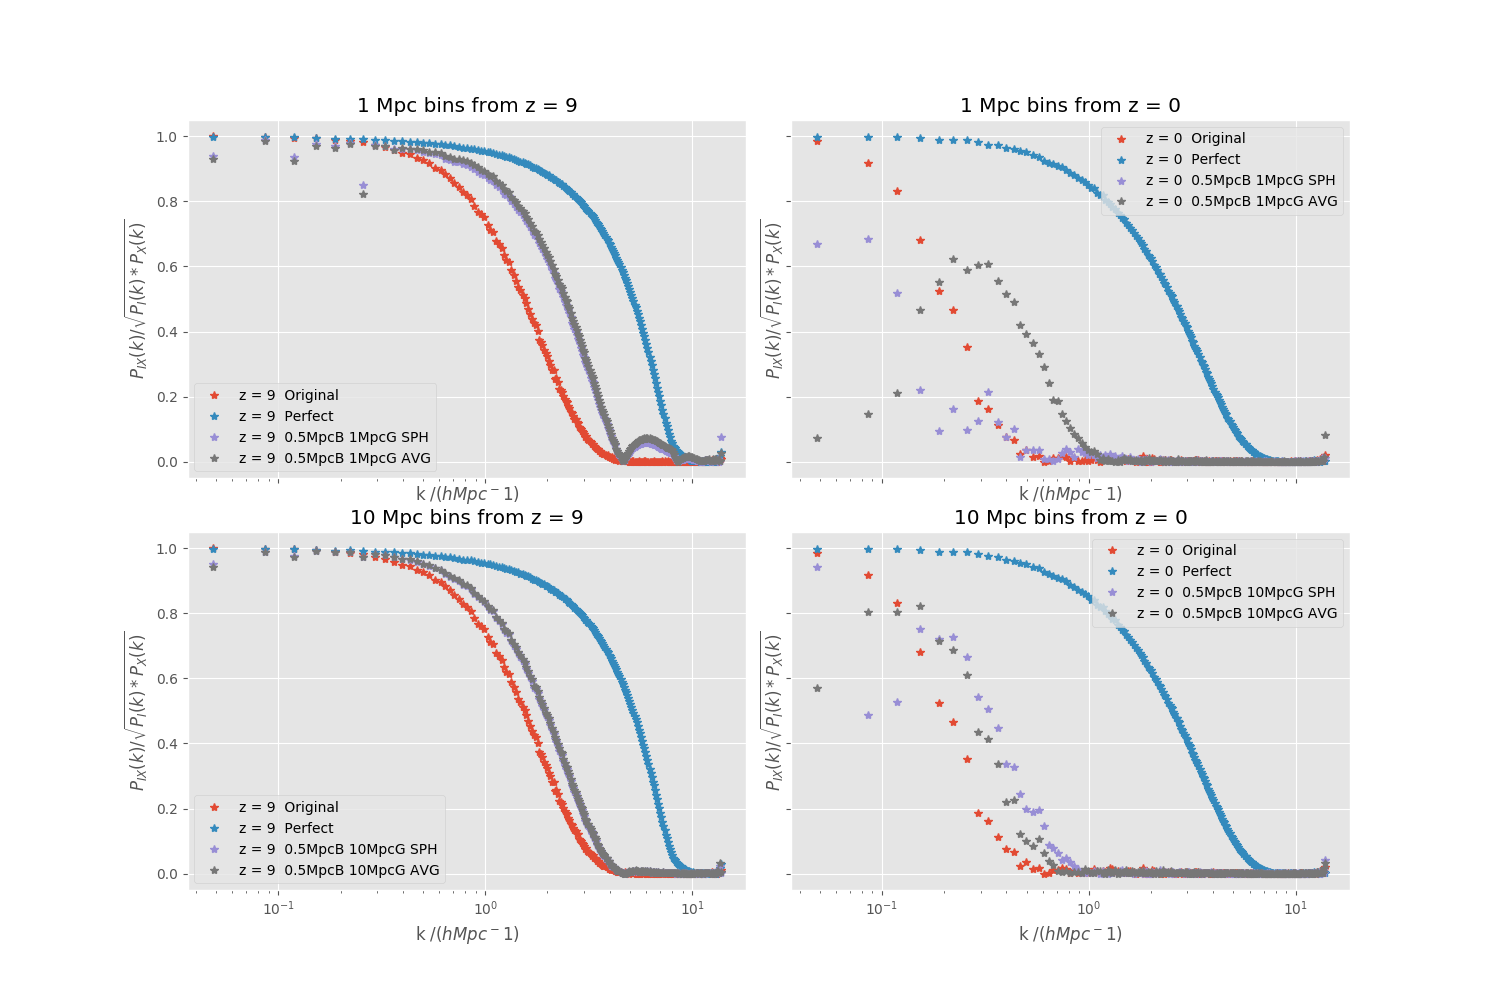
\includegraphics[width=1\columnwidth]{images/crossSpectra/Spec_6_filt.png}%
    
%     \caption{
%         Cross spectra of realistic reconstructions from redshift 9 and 0, using 1 Mpc and 10 Mpc bins to smooth velocities. In this case the average was taken across 0.5 Mpc bins (using the two methods presented above), and then a Gaussian Filter with standard deviation of 1 Mpc and 10 Mpc respectively was applied.
%     }
    
%     \label{fig:9}
% \end{figure}


\section{Analysis}

\todo[inline]{Talk about the results for different averaging methods and Bin Sizes.}

% \begin{figure}
%     \centering
%     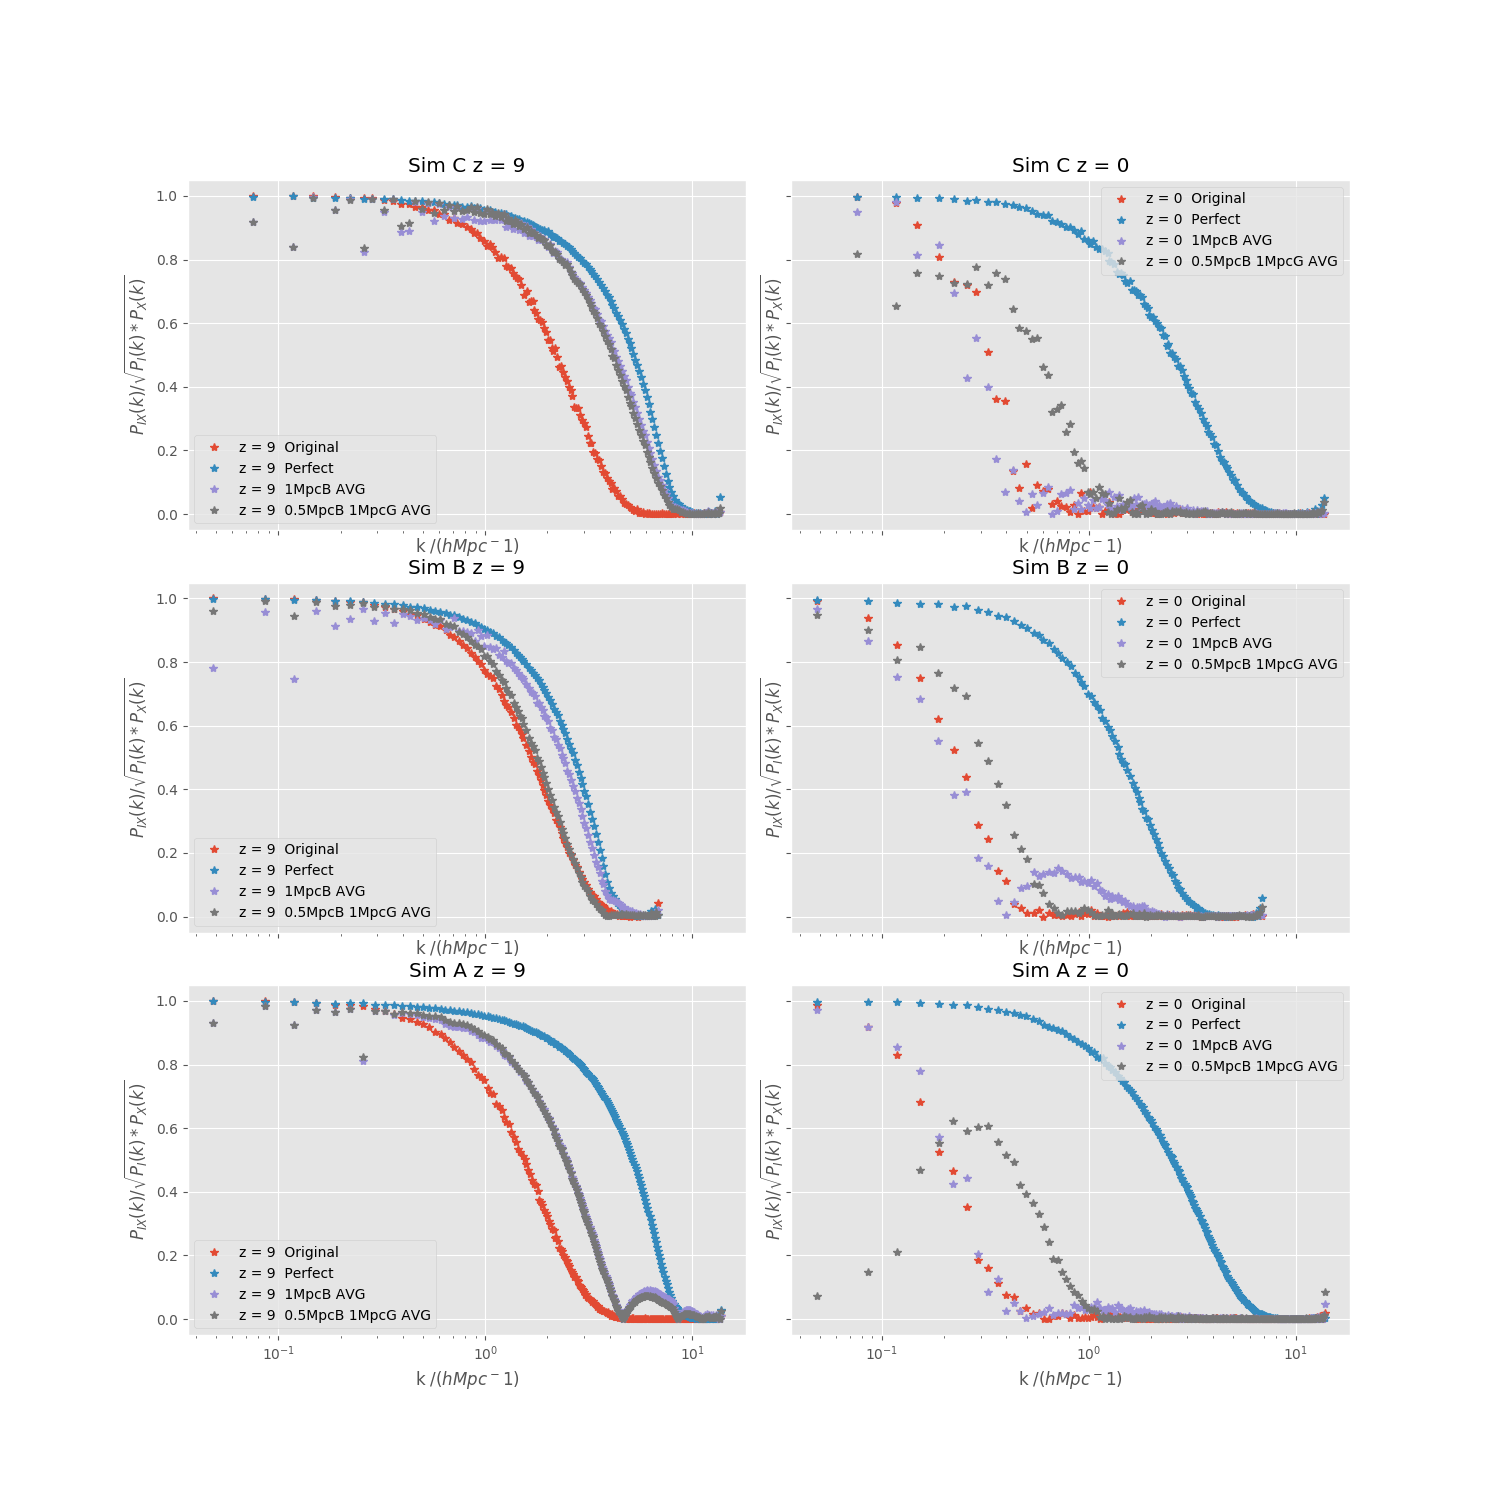
\includegraphics[width=1\columnwidth]{images/crossSpectra/Spec_8_sims.png}%
    
%     \caption{
%         Cross spectra of realistic reconstructions from redshift 9 and 0 across the 3 simulations. Velocities were averaged over 1 Mpc scales using normal averaging of all the particles in each bin.
%     }
    
%     \label{fig:10}
% \end{figure}

% \begin{figure}
%     \centering
%     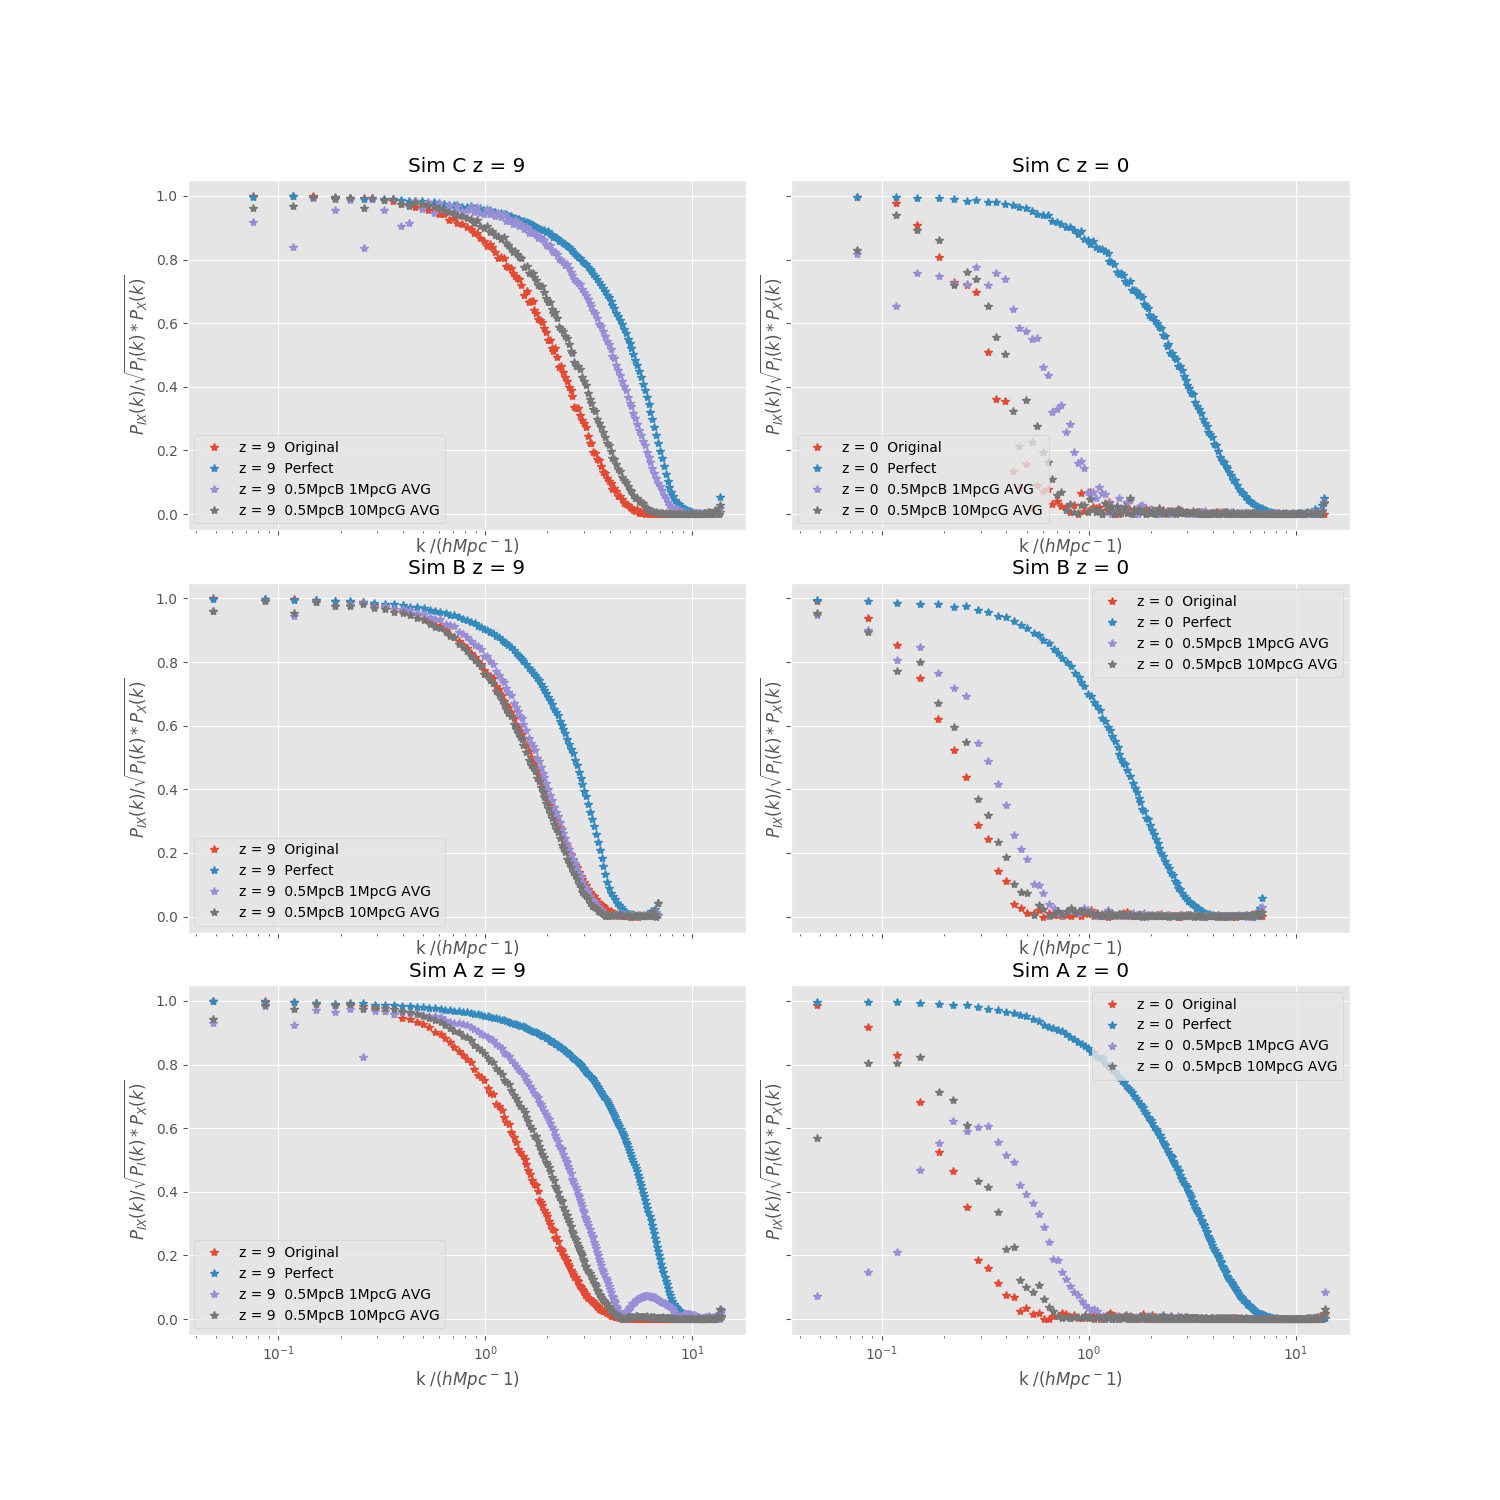
\includegraphics[width=1\columnwidth]{images/crossSpectra/Spec_9_sims.png}%
    
%     \caption{
%         Cross spectra of realistic reconstructions from redshift 9 and 0 across the 3 simulations. Velocities were averaged over 1 Mpc and 10 Mpc scales using normal averaging of all the particles in each bin.
%     }
    
%     \label{fig:11}
% \end{figure}

